\documentclass[11pt, oneside]{article} 
\usepackage{geometry}
\geometry{letterpaper} 
\usepackage{graphicx}
	
\usepackage{amssymb}
\usepackage{amsmath}
\usepackage{parskip}
\usepackage{color}
\usepackage{hyperref}

\graphicspath{{/Users/telliott/Github/precalculus/fig/}}
% \begin{center} \includegraphics [scale=0.4] {gauss3.png} \end{center}

\title{Circle analytically}
\date{}

\begin{document}
\maketitle
\Large

We now consider what are called quadratic forms, as distinguished from linear equations (i.e., for lines).  The quadratics contain a squared term (or a term that mixes $x$ and $y$).  
\begin{center} 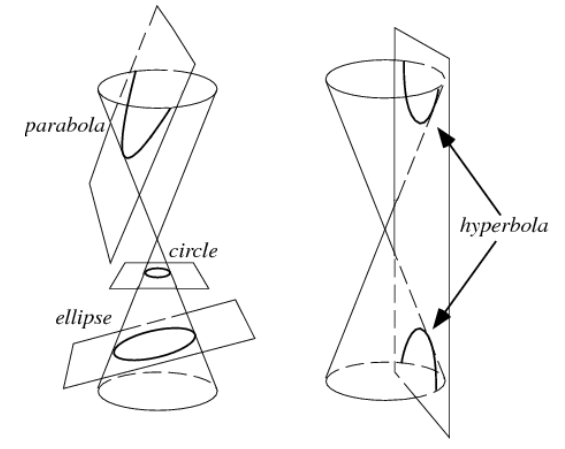
\includegraphics [scale=0.5] {conic_sections.png} \end{center}
The simplest example is the equation for a unit circle centered at the origin:
\[ x^2 + y^2 = 1 \]

Pythagoras tells us that for a point $(x,y)$, the square of the distance from the origin is $x^2 + y^2$.  This equation describes all the points whose distance from the origin is equal to $\sqrt{1} = 1$.  But all  the points equi-distant to a point form a circle.  We generalize
\[ x^2 + y^2 = r^2 \]

It is clear that when $y = 0$, $x = \pm \ r$.  $r$ is the radius of the circle.

Now, what happens if we displace the unit circle from the origin so its center is at $(1,0)$?  What this amounts to is adding $1$ to the $x$ value of every point.  If we solve for $x$
\[ x = \sqrt{1 - y^2} \]
and then add $1$
\[ x = \sqrt{1 - y^2} + 1 \]
\[ (x - 1)^2 = 1 - y^2 \]
\[ (x - 1)^2 + y^2 = 1 \]

Or, more generally 
\[ (x - h)^2 + (y - k)^2 = r^2 \]
where the origin of the circle is at $(h,k)$.  

Multiplying out:
\[ x^2 - 2hx + h^2 + y^2 - 2ky + k^2 = r^2 \]
\[ x^2  + y^2 - 2hx - 2ky + (h^2 + k^2 - r^2) \]

Comparing to the most general form for a quadratic
\[ Ax^2 + By^2 + Cxy + Dx + Ey + F = 0 \]

We see that
\[ A = 1, \ \ \ \ B=1, \ \ \ \ C = 0 \]
and in fact, this is true for all circles.  (If $A = B \ne 1$, just divide all the terms by $A$).

Moreover
\[ D = - 2h, \ \ \ \ E = - 2k, \ \ \ \ F = h^2 + k^2 - r^2 \]

This equation can help us solve the following problem from Hamming:  find the equation of the circle that passes through the following three points:
\[ (-1,1), (1,1), (2,3) \]

\begin{center} 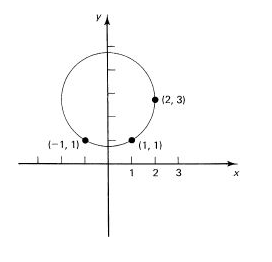
\includegraphics [scale=0.9] {Hamming_6_2_2.png} \end{center}
We write
\[ x^2 + y^2 + Dx + Ey + F = 0 \]
From the values of $x$ and $y$ at each of the three points we get
\[ 1 + 1 - D + E + F = 0 \]
\[ 1 + 1 + D + E + F = 0 \]
\[ 4 + 9 + 2D + 3E + F = 0 \]
Three equations in three unknowns.  We can do that.

Adding the first two equations together:
\[ 4 + 2(E + F) = 0 \]
so $E + F = -2$.

Subtracting the first two equations (or substituting the result for $E + F$) tells us that $D = 0$.

Adding $(-3)$ times the second equation to the third gives:
\[ 1 + 6 - D - 2F = 0 \]
\[ 7 - 2F = 0 \]
$F = 7/2$, and since $E + F = -2$, $E = -11/2$.

So the solution is
\[ x^2 + y^2 - \frac{11}{2} y + \frac{7}{2} = 0 \]

You can check that it works for all three points:
\[ (-1,1), (1,1), (2,3) \]
The first two are easy, while the third gives
\[ 4 + 9 - \frac{11}{2} 3 + \frac{7}{2} = 0 \]
\[ 8 + 18 - 33 + 7 = 0 \]
which looks correct.

\section*{completing the square}

We can improve this by completing the square.  We see that
\[ y^2 - \frac{11}{2} y + ( \frac{11}{4})^2 = (y - \frac{11}{4})^2 \]

We must add that back to the right-hand side of the original to obtain:
\[ x^2 +  (y - \frac{11}{4})^2 =  ( \frac{11}{4})^2 - \frac{7}{2} \]

The center is at $(0,11/4)$.  The radius doesn't come out cleanly but $r^2$ is
\[ \frac{121}{16} - \frac{56}{16} = \frac{65}{16} \]
so $r$ is slightly more than $2$.

Or recall that we had:
\[ D = - 2h, \ \ \ \ E = - 2k, \ \ \ \ F = h^2 + k^2 - r^2 \]

From this, we have that $h = 0$ and $k = -E/2 = 11/4$, and the radius is more complicated, as we said.

\subsection*{plane geometry}

We can check our work by solving the problem using a technique from plane geometry.  Again, we want the circle passing through three points:
\[ (-1,1), (1,1), (2,3) \]

Take two of the points to be placed on a circle and construct the line segment joining them (a chord of the circle).  Find the midpoint of the chord and erect a perpendicular bisector through the midpoint.  Now, every point lying on the bisector is equidistant from the two starting points.  Proof:  draw the two triangles including that point, the two starting points and the midpoint of the bisector.  The two triangles are congruent.  Here is the general picture.

\begin{center} 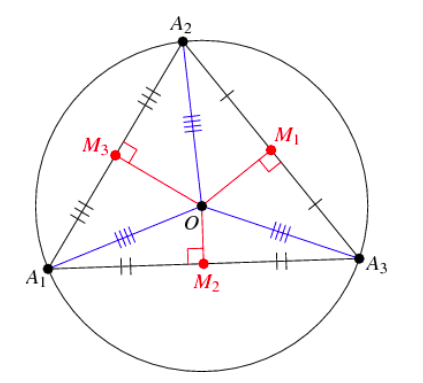
\includegraphics [scale=0.6] {three_point_circle2.png} \end{center}
It's a bit trickier to prove that \emph{every} point that is equidistant from the two points lies on the bisector.  We assume that.  

Since every point that is equidistant from the two points lies on the bisector, the radius of the circle lies on the bisector.  

Then, erect a perpendicular bisector of a chord joining another pair chosen from the three points.  This new bisector and the first one meet at the center of the circle.

In our case two points $(-1,1), (1,1)$ are symmetric about the $y$-axis.  Therefore it is clear that the perpendicular bisector for these two points is the $y$-axis.
\begin{center} 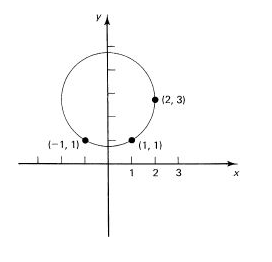
\includegraphics [scale=0.9] {Hamming_6_2_2.png} \end{center}
For the second bisector, form the vector between $(1,1)$ and $(2,3)$ as $\mathbf{v} = \langle 1,2 \rangle$.  The midpoint is at $(1,1) + \mathbf{v}/2 = (3/2, 2)$.

The slope of the bisector is the negative inverse of the slope for the chord which is $- 1/2$ so the equation of the bisector is
\[ y - y_0 = -\frac{1}{2} (x - x_0) \]
Plugging in the point that we know, we obtain
\[ y - 2 = -\frac{1}{2} (x - 3/2) \]
We want to solve for $y$ when $x = 0$, crossing the first bisector, the $y$-axis
\[ y - 2 = -\frac{1}{2} (- 3/2) \]
\[ y = \frac{11}{4} \]
So the center is at $(0,11/4)$, which matches what we had before.  We compute the distance to one of the points $(1,1)$ as
\[ d = \sqrt{1^2 + (11/4 - 1)^2} = \sqrt{1 + 49/16} \]
which also matches our previous result.

\subsection*{quadratics}

The technique of completing the square comes from the standard equation
\[ (x + p)^2 = x^2 + 2px + p^2 \]

We run into problems where we have the $2px$ but not the $p^2$.  For example
\[ x^2 + y^2 + Dx + F = 0 \]

Focus on
\[ x^2 + Dx \] 
we want to turn this into 
\[ (x + \text{something})^2 \]
if $D$ is like $2p$ we need to add something like $p^2$:
\[ x + Dx + \frac{D^2}{4} \]
\[ = (x + \frac{D}{2})^2 \]
Since we added $D^2/4$ on the left, we must also add it on the right.  We obtain
\[ (x + \frac{D}{2})^2 + y^2 + F = \frac{D^2}{4} \]

You don't believe me?  Multiply it out
\[ x^2 + Dx +  \frac{D^2}{4} + y^2 + F = \frac{D^2}{4} \]
To form $(x + D/2)^2$ on the left-hand side, we added $D^2/4$ (what we needed) to both sides.

Again, the general equation for a quadratic is
\[ Ax^2 + Bxy + Cy^2 + Dx + Ey + F = 0 \]

In starting to work with one of these, the first thing to do is to see if there is a term which "mixes" $x$ and $y$, that is, whether there is some term like $Bxy$.  If there is, we might think about rotating the curve so that it is in a standard orientation.  

We'll talk about how to do that \hyperlink{rotation}{\textbf{here}}, in the context of the ellipse.  However, the approach is general.

Let us assume we've done that, we relabel the new $A$, $C$ etc. and assume here that $B = 0$.

Once in standard orientation, the next thing we might do is to translate the quadratic so that it is centered on the origin.  We do that by completing the square for both $x$ and $y$.  We did some of that in this chapter, and we'll talk more about it \hyperlink{completing_the_square}{\textbf{here}}
in the context of the parabola.  Once again, however, the approach is general.

Cases:

$\bullet$  Both $A$ and $C$ present, and $F < 0$.  If

$\ \ \circ$  $A$ and $C$ are both $> 0$:  it's an ellipse.

$\ \ \circ$  $A$ and $C$ are of opposite signs:  it's a hyperbola.

$\bullet$  $A$, $C$ and $F$ are all negative:  it's imaginary.

$\bullet$  Only one squared term is present, but we still have the other variable

$Ax^2 + Ey + F = 0$  :  it's a hyperbola.

Not every quadratic equation gives a conic.  Some are "degenerate".  For example, having done all the right manipulations, we might end up with something like
\[ A'(x-h)^2 + B'(y-k)^2 = 0 \]
which has only $x=h$ and $y=k$ as a solution.  It's a point.

\begin{center} 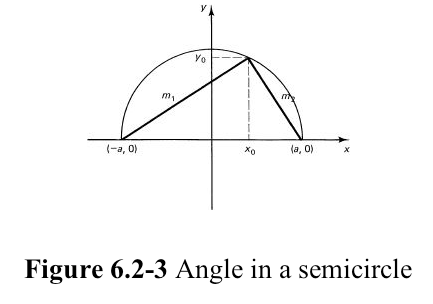
\includegraphics [scale=0.8] {Hamming_6_2_3.png} \end{center}

Here is another problem from Hamming.  We need to prove that the angle above is a right angle.  Suppose the equation of the circle is 
\[ x^2 + y^2 = a^2 \]
The point on the circle is $(x_0,y_0)$.

Our first solution uses slopes and points.  The line from $(-a,0)$ to $(x_0,y_0)$ has slope
\[ m_1 = \frac{y_0}{x_0 + a} \]
The line from $(a,0)$ to $(x_0,y_0)$ has slope
\[  m_2 = \frac{y_0}{a - x_0} \]
Two lines meet at a right angle if the product of their slopes is equal to $-1$.
\[ m_1 m_2 = \frac{y_0}{x_0 + a} \ \frac{y_0}{a - x_0} \]
\[ = \frac{y_0^2}{a^2 - x_0^2} = \frac{y_0^2}{x_0^2 + y_0^2 - x_0^2} = - 1 \]

This was not pretty, it's just good exercise.  

And here is a proof using vectors and the dot product.  Consider the semicircle centered on the origin with radius $a$, so the ends of the diameter are at $(x = \pm \ a, 0)$.  

Form the vectors from those ends to an arbitrary point $(x,y)$ on the perimeter:
\[ \mathbf{u} = \ \langle x + a, y \rangle \]
\[ \mathbf{v} = \ \langle x - a, y \rangle \]
Notice that
\[  \mathbf{u} \cdot  \mathbf{v} = (x + a)(x - a) + y^2 \]
\[ = x^2 -a^2 + y^2 = 0 \]
because $x^2 + y^2 = a^2$ for any point on the circle.

As our last example, consider the problem of finding the equation of a line tangent to a circle that goes through some arbitrary point $b$.
\begin{center} 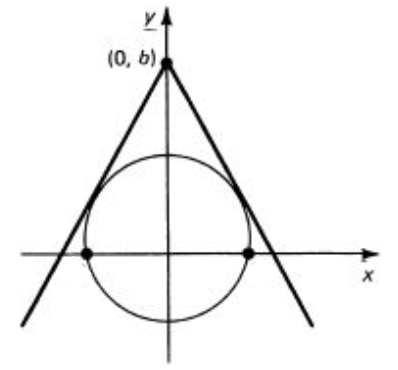
\includegraphics [scale=0.4] {Hamming_6_3_1_rev.png} \end{center}

We take the circle to have radius $a$ and be centered at the origin.  We take the point $b$ to be on the $y$-axis.  The equation of the line on the right side is
\[ \frac{y - y_0}{x - x_0} = m = \frac{y - b}{x} \]
\[ y = mx + b \]
(well, of course).

For the point or points where the line intersects the circle we also have
\[ y = \sqrt{a^2 - x^2} \]
\[ \sqrt{a^2 - x^2} =  mx + b \]
\[ a^2 - x^2 = m^2x^2 + 2bmx + b^2 \]
\[ (m^2 + 1)x^2 + 2bmx + b^2 - a^2 = 0 \]
From the quadratic equation:
\[ x = \frac{-2bm \pm \sqrt{4b^2m^2 - 4(m^2 + 1)(b^2 - a^2)}}{2(m^2 + 1)} \]
We are looking for the case where there is a single solution so the discriminant under the square root must be equal to zero:
\[ 4b^2m^2 = 4(m^2 + 1)(b^2 - a^2) \]
\[ m^2b^2 = m^2b^2 - m^2a^2 + b^2 - a^2 \]
\[ 0 = -m^2a^2 + b^2 - a^2 \]
\[ m = \pm  \frac{\sqrt{b^2 - a^2}}{a}  \]
This makes sense since if $a=b$ the single tangent should be horizontal with zero slope.  Notice that if $a^2 > b^2$ there is no real solution.  This corresponds to having $b$ inside the circle.

\end{document}